\chapter{实数理论}

\section{自然数集的构造与公理化}

回顾第一章的练习1.5 a), 如果将$x \mapsto x^+$的过程视作后继映射$S: N_0 \to N_0$, 我们在von Neumann构造的自然数集中实际上证明了以下四件事情: 

i) $x=y \Rightarrow x^+ = y^+$, 即该映射的定义是合理的; 

ii) $\forall x \in N_0, ~x^+ \neq \varnothing$, 即$\varnothing \notin S(N_0)$; 

iii) $(A \subseteq N_0) \wedge (\varnothing \in A) \wedge (\forall x \in A, ~x^+ \in A) \Rightarrow A=N_0$, 即如果自然数集的子集也是归纳集, 那么该子集就是自然数集本身; 

iv) $x^+=y^+ \Rightarrow x=y$, 即$S$是一个单射.

以上四件事情在熟知的那个自然数集中似乎也是成立的. 那么, 能否将所有具有如上性质的集合都考虑为自然数集呢? 具体地讲, 我们需要一些公理.

\begin{axiom}{Peano公理}
	设集合$X$及其上的一个映射$S$. 若$X$和$S$满足
	\begin{enumerate}
		\item $x \in X$; 
		\item $x \notin S(X)$; 
		\item $S$是一个单射; 
		\item $X$对于$S$是封闭的; 
		\item (极小性公设)对任意$A \subseteq X$都有: 若$x \in A$且$A$对$S$封闭, 则$A=X$. 
	\end{enumerate}
	则$X$是自然数集. 
\end{axiom}
\begin{remark}
	一般称$x$为初始元素, $S$为后继映射. 由$(X, S, x)$构成的组称为一个Peano系统. 一般记$0: =x$.
\end{remark}

如果第二条不成立, 可能会存在某个元素的后继为初始元素, 从而形成循环; 如果第三条不成立, 则有可能两个元素的后继是同样的; 若第四条不成立, 则会有某个元素后面没有后继元素; 第五条也被称为归纳原理, 用处在于排除多链的情况. 

\begin{figure}[h!]
	\centering
	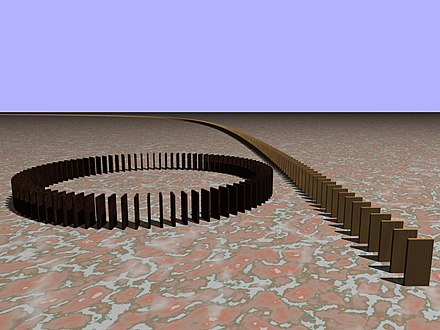
\includegraphics[width=6cm]{attachment/440px-Domino_effect_visualizing_exclusion_of_junk_term_by_induction_axiom.jpg}
	\caption{多链示意图, 深色的骨牌是我们不想要的. 图源Wikipedia}
\end{figure}



1.5 a)的四条结论和$N_0$的定义足以说明$N_0=\mathbb{N}$.也即, 通过定义$\mathbb{N}$是最小的归纳集和利用Peano公理定义$\mathbb{N}$是完全等价的.

定义前10个自然数的符号分别为$0, 1, 2, 3, 4, 5, 6, 7, 8, 9$.

这里再声明一次(第一)数学归纳法, 方便后面使用.

\begin{theorem}{第一数学归纳法} \label{thm:diyigvna}
	设$P(n)$是关于自然数$n$的一个性质. 如果
	\begin{enumerate}
		\item 当$n=0$时, $P(n)$成立; 
		\item 由$P(n)$成立可以推出$P(n+1)$成立.
	\end{enumerate}
	那么, 对任意$n \in \mathbb{N}$, $P(n)$都成立.
\end{theorem}
\begin{proof}
	这是极小性公设的直接推论. 
\end{proof}

\subsection{自然数集上的加法}

自然数中可以一步完成的加法已经有明确的定义: $n+0=n, ~n+1=S(n)$.从而可以归纳地定义完全的加法.

\begin{definition}{自然数集上的加法}
	设自然数集$\mathbb{N}$, $S$是$\mathbb{N}$上的后继映射.定义自然数集上的\textit{加法}(addition)映射为满足如下条件的映射$+: \mathbb{N}^2 \to \mathbb{N}, ~(n, m) \to n+m$: 
	\begin{enumerate}
		\item $n+0=n$.
		\item $n+S(m)=S(n+m)$.
	\end{enumerate}
\end{definition}

既然加法是归纳定义, 我们同样可以利用归纳法证明加法的诸多性质: (证明略去, 后文亦如此)

\begin{proposition}{自然数的加法运算律}
	对于任意的$a, b, c \in \mathbb{N}$, 都有
	\begin{enumerate}
		\item (结合律)~$(a+b)+c = a+(b+c)$.
		\item (交换律)~$a+b=b+a$.
		\item (消去律)~$a+c=b+c \Leftrightarrow a=b$.
	\end{enumerate}
\end{proposition}

为了得到熟悉的减法定义与运算律, 要先明确构造的可行性: (其中$\mathbb{N}^* : = \mathbb{N} - \{ 0 \}$.)

\begin{proposition}{} \label{pro:jmfagzzckexkxk}
	对任意$b \in \mathbb{N}^*$, 存在$a \in \mathbb{N}$使得$S(a)=b$.
\end{proposition}

\subsection{自然数集中的序关系}

类似于利用$a=kb$定义$b \mid a$这一序关系, 可以利用加法来定义自然数的序关系.

\begin{definition}{自然数集中的序关系}
	设$a, b \in \mathbb{N}$.如果存在$k \in \mathbb{N}$使得$a+k=b$, 则称$a$\textit{小于等于}(less than or equal to)$b$, 记作$a \leq b$.特别地, 若$a \leq b$且$a \neq b$, 则称$a$\textit{小于}(less than), 记作$a<b$.
\end{definition}

自然数集中的小于等于关系是一个全序关系, 利用归纳法容易验证其满足传递性、反对称性、完全性.

关于小于关系, 还有一个类似完全性的命题: 

\begin{proposition}{自然数集的三歧性}
	对于任意$a, b \in \mathbb{N}$, 下列命题中恰有一个成立: 
	\begin{center}
		$a<b,  \qquad a=b,  \qquad a>b.$
	\end{center}
\end{proposition}


\begin{proposition}{自然数的加法保序性}
	对于任意$a, b, c \in \mathbb{N}$, 有
	\begin{center}
		$a+c \geq b+c \Leftrightarrow a \geq b.$
	\end{center}
\end{proposition}

自然数还有一项重要的性质: 

\begin{proposition}{自然数的离散性}
	对于任意$a, b \in \mathbb{N}$都有
	\begin{center}
		$a>b \Leftrightarrow a \geq S(b).$
	\end{center}
\end{proposition}

现在, 我们对数学归纳法做一些集中的研究.

\begin{theorem}{第二数学归纳法} \label{thm:diergvna}
	设$P(n)$是关于自然数$n$的一个性质.如果
	\begin{enumerate}
		\item 当$n=0$时, $P$成立; 
		\item 假设$n \leq k$时$P(n)$都成立, 则当$P(k+1)$也成立.
	\end{enumerate}
	那么, 对任意$n \in \mathbb{N}$, $P(n)$都成立.
\end{theorem}

\begin{theorem}{良序定理} \label{thm:llxu}
	对于任意非空集合$A \subseteq \mathbb{N}$, $A$中都存在一个元素$M$, 使得$\forall a \in A, ~a \geq M$.
\end{theorem}
\begin{proof}
	假设对任意的$M$, 总存在某个$a \in A$使得$a < M$. 下面归纳证明$A^c = \mathbb{N}$. 
	
	(i)假设$0 \in A$, 又由于任意自然数$n$有$n \geq 0$(利用命题\ref{pro:jmfagzzckexkxk}结合归纳法可以证明), 于是与$A$的定义矛盾, 故$0 \notin A$, 那么$0 \in A^c$. 
	
	(ii)假设对任意的$n \leq k$, 都有$n \in A^c$即$n \notin A$, 那么假若$k+1 \in A$, 由于$n \leq k < k+1$, 这与$A$的定义矛盾, 所以$k+1 \notin A$, 从而$k+1 \in A^c$. 
	
	由第二数学归纳法可知, $A^c = \mathbb{N}$, 即$A = \varnothing$, 与假设矛盾. 所以原命题成立.
\end{proof}

反过来, 利用反证法也能说明良序定理可以推导第一数学归纳法.从而, 定理\ref{thm:diyigvna}, \ref{thm:diergvna}, \ref{thm:llxu}是等价的.

\subsection{自然数集中的乘法}

仿照加法, 继续归纳定义乘法: 

\begin{definition}{自然数集上的乘法}
	设自然数集$\mathbb{N}$, $S$是$\mathbb{N}$上的后继映射. 定义自然数集上的\textit{乘法}(multiplication)映射为满足如下条件的映射$\times : \mathbb{N}^2 \to \mathbb{N}, ~(n, m) \to n \times m$: 
	\begin{enumerate}
		\item $n\times 0=0$.
		\item $n\times S(m)=n\times m+n$.
	\end{enumerate}
\end{definition}

如此定义的乘法和我们心中的模样如出一辙: 利用归纳法容易证明$n \times m = \overbrace{n+n+\cdots +n}^{m~ \text{times}}$. 在获得乘法交换律之前, 注意$m$和$n$的顺序! 

利用归纳法, 不难证明下列命题: 

\begin{proposition}{自然数的乘法运算性质}
	对于任意的$a, b, c \in \mathbb{N}$, 都有
	\begin{enumerate}
		\item (分配律)~$(a+b)c = ab+ac$.
		\item (单位元)~$a \times 0 = 0 \times a = 0, ~a \times 1 = 1 \times n = n$.
		\item (交换律)~$ab=ba$.
		\item (结合律)~$(ab)c=a(bc)$.
	\end{enumerate}
\end{proposition}

为了得到消去律, 还要再做些准备: 

\begin{proposition}{自然数的乘法无零因子律}
	对任意$a, b \in \mathbb{N}$, $ab=0$当且仅当$a=0$或$b=0$.
\end{proposition}

\begin{proposition}{自然数的乘法保序性}
	对于任意$a, b, c \in \mathbb{N}$, 其中$c \neq 0$, 总有
	\begin{center}
		$a>b \Leftrightarrow ac>bc.$
	\end{center}
\end{proposition}

结合乘法保序性, 利用反证法可以得到乘法消去律.

\begin{corollary}{自然数的乘法消去律}
	对于任意$a, b, c \in \mathbb{N}$, 其中$c \neq 0$, 总有
	\begin{center}
		$a=b \Leftrightarrow ac=bc.$
	\end{center}
\end{corollary}

乘法是对加法的累积, 次幂则是对乘法的累积.

\begin{definition}{自然数的次幂}
	设自然数集$\mathbb{N}$, $S$是$\mathbb{N}$上的后继映射.定义自然数集上的\textit{指数}(exponentiation)映射为满足如下条件的映射$\sigma : \mathbb{N}^2-\{ (0, 0) \} \to \mathbb{N}, ~(n, m) \to n^m$: 
	\begin{enumerate}
		\item 对于$n \neq 0$, 有$n^0=1$, $n^{S(m)}=n^m \times n$.
		\item 对于$n \neq 0$, 若$m \neq 0$则$n^m=0$.
	\end{enumerate}
\end{definition}

同样利用归纳法可以证明, $n^m = \overbrace{n\times n\times \cdots \times n}^{m~ \text{times}}$.


\newpage
\section{整数环的构造}

在自然数集中定义减法时, 我们会注意到, 并不是所有自然数相减都会得到自然数, 也即自然数集对加法逆元不封闭. 为了保证封闭, 尝试在自然数的基础上构造整数.

通过自然数的差来构造整数是一个好思路. 不过, 这种相对差量不能保证唯一性, 即整数$a$可能通过任意的$(a+k)-k$得到. 从而, 可以考虑用等价类的方法定义整数. 

\begin{definition}{整数集}
	在$\mathbb{N}^2$上定义等价关系$\sim$如下: $$(a_1, b_1) \sim (a_2, b_2) : \Leftrightarrow a_1+b_2=a_2+b_1.$$
	将每个等价类视作一个\textit{整数}(integer), 所有等价类构成的集合视作整数集, 记作$\mathbb{Z}$.
\end{definition}

接着定义整数集里的加法与乘法: 

\begin{definition}{整数集的加法和乘法}
	规定加法: $$[(a_1, b_1)]_{\sim} + [(a_2, b_2)]_{\sim} : = [(a_1+b_1, b_1+b_2)]_{\sim}.$$
	乘法: 
	$$[(a_1, b_1)]_{\sim} \times [(a_2, b_2)]_{\sim} : = [(a_1a_2+b_1b_2, a_1b_2+a_2b_1)]_{\sim}.$$
\end{definition}

如此定义的加法和乘法显然是良定义的. 

接着可以得到理想中的结果: 上述定义的整数集同构于自然数集的某个母集. 或者反过来更好描述: 自然数集同构(存在双射并保持代数结构)于整数集的某个子集. 

\begin{proposition}{}
	记$\tilde{\mathbb{N}}: =\{ [(a, b)]_{\sim} \in \mathbb{Z}: a \leq b \}$.那么存在双射$$\sigma : \tilde{\mathbb{N}} \to \mathbb{N}, ~[(a, b)]_{\sim} \mapsto a-b, $$
	并且有$$\sigma (\alpha) + \sigma (\beta) = \sigma (\alpha + \beta), \quad \sigma (\alpha) \times \sigma (\beta) = \sigma (\alpha  \beta)$$
	对于所有$\alpha , \beta \in \tilde{\mathbb{N}}$成立.
\end{proposition}

大一统的基业既已完成, 我们终于得以见到熟悉的记号了: 

\begin{definition}{}
	对于$[a, b]_{\sim} \in \mathbb{Z}$, 由自然数的三歧性可知$a>b, a=b$或$a<b$. 
	\begin{itemize}
		\item 当$a>b$时, 记$n: =[(a, b)]_{\sim}$, 其中$n$是满足$a=b+n$的自然数, 此时称$n$为\textit{正的}(positive). 
		\item 当$a<b$时, 记$-n: =[(a, b)]_{\sim}$, 其中$n$是满足$b=a+n$的自然数, 此时称$-n$为\textit{负的}(negative). 
		\item 当$a=b$时, 记$0: =[(a, b)]_{\sim}$, 这里$0$是自然数集的最小元素.
	\end{itemize}
\end{definition}

将自然数集的一些性质推广, 容易得到: 

\begin{proposition}{整数运算的性质}
	(1) 单位元$$\forall a \in \Z ,  a + 0 = 0+ a = a ,  1 a = a 1 = a .$$
	(2) 加法逆元$$\forall a \in \Z ,  \exists ! b \in \Z ,  a + b = 0 .$$
	(3) 结合性质$$\forall a ,  b ,  c \in \Z ,  (a + b) + c = a + (b + c) ,  (a b) c = a (b c) .$$
	(4) 交换性质$$\forall a ,  b \in \Z ,  a + b = b + a ,  a b = b a .$$
	(5) 分配性质$$\forall c ,  a ,  b \in \Z ,  c (a + b) = c a + c b, (a+b)c=ac+bc .$$
\end{proposition}

\begin{proposition}{整数的乘法无零因子律}
	对任意$a, b \in \Z$, $ab=0$当且仅当$a=0$或$b=0$.
\end{proposition}

\begin{corollary}{整数的乘法消去律}
	对于任意$a, b, c \in \Z$, 其中$c \neq 0$, 总有$$a=b \Leftrightarrow ac=bc.$$
\end{corollary}

实际上, 如果集合$G$上的一个运算$\bigcdot$满足单位元、逆元、结合性质, 我们就称$(G,\bigcdot )$是一个\textit{群}(group). 如果$\bigcdot$还满足交换性质, 则称$(G,\bigcdot )$是一个\textit{交换群}(commutative group)或\textit{Abel群}(Abel group).

在一个集合上, 往往只定义了加法, 例如平面向量(因为平面向量之间的内积和外积都不封闭). 有些时候可以得到具有加法和乘法的集合, 例如所有映射构成的集合, 但是它们的乘法不满足交换性质. 

对于定义了加法和乘法的集合, 可以得到所谓环的概念: 

\begin{axiom}{环}
	设非空集合$R$, 若$R$上定义了加法$+$和乘法$\bigcdot$并满足: 
	\begin{enumerate}
		\item $(R,+)$构成Abel群; 
		\item $\bigcdot$满足结合性质; 
		\item $\bigcdot$对$+$有分配性质. 
	\end{enumerate}
	则称$(R,+,\bigcdot )$是一个\textit{环}(ring).
\end{axiom}

整数集$(\Z ,+,\times )$显然是一个环. 由两个集合间所有映射构成的集合也是一个环. 

考虑一整个代数结构而不是单纯的特例, 可以方便我们迁移应用. 例如, 整数环与一元多项式环的性质非常相似, 所以它们共享很多定理与定义(带余除法定理, 素数和既约多项式等等). 

\begin{definition}{整数的减法}
	记$-n$表示整数$n$的加法逆元.则定义减法映射$-: \Z ^2 \to \Z , (a, b) \mapsto a-b$, 满足$$a-b: =a+(-b).$$
\end{definition}

良定义是显然的.

\begin{definition}{整数的序关系}
	对于$[(a_1, b_1)]_{\sim}, [(a_2, b_2)]_{\sim} \in \Z$, 定义它们的序关系: $$[(a_1, b_1)]_{\sim} \leq [(a_2, b_2)]_{\sim} \Leftrightarrow a_1+b_2 \leq b_1+a_2.$$
\end{definition}

注意$n$为负就等价于$n<0$.

容易验证, 整数间的序关系是一个全序关系, 并且自然数的三歧性在这里同样使用.

整数间的序关系比较复杂, 例如对于负数$c$, $a \leq b \Leftrightarrow ac \geq bc$. 这些熟知性质就不一一罗列了.

\newpage
\section{有理数域的构造}

从自然数集扩大得到的整数集虽然对减法封闭了, 它对除法还是不封闭. 用同样的方式可以将整数集扩大到有理数集.

\begin{definition}{有理数集}
	在$\mathbb{Z}^2$上定义等价关系$\sim$如下: $$(a_1, b_1) \sim (a_2, b_2) : \Leftrightarrow a_1b_2=a_2b_1.$$
	将每个等价类$[(a, b)]_{\sim}$视作一个\textit{有理数}(rational number), 记作$a/b$. 所有等价类构成的集合视作有理数集, 记作$\mathbb{Q}$.
\end{definition}

由定义可知, $(a, b)\in a/b$等价于$(ka, kb) \in a/b$, 这里$k$为任意非零整数. 

\begin{definition}{有理数集的加法和乘法}
	规定加法: $$\frac{a_1}{b_1} + \frac{a_2}{b_2} = \frac{a_1b_2+a_2b_1}{b_1b_2}.$$
	乘法: 
	$$\frac{a_1}{b_1} \times \frac{a_2}{b_2} = \frac{a_1a_2}{b_1b_2}.$$
\end{definition}

只需注意到, $\mathbb{Q}$中的加法单位元为$0/1$, 乘法单位元为$1/1$, 容易验证$(\mathbb{Q}, + ,\times )$也是一个环, 并且乘法满足单位元、逆元、交换性质.

类似地, 可以将$\Z$与$\mathbb{Q}$中的某个子集同构. (这里$b \mid a, ~a, b \in \Z$表示存在$n \in \Z$使得$a=nb$.)

\begin{proposition}{}
	记$\tilde{\mathbb{Z}}: =\{ a/b \in \mathbb{Q}: b \mid a \}$.那么存在双射$$\sigma : \tilde{\mathbb{Z}} \to \mathbb{Q}, a/b \mapsto n, $$
	并且有$$\sigma (\alpha) + \sigma (\beta) = \sigma (\alpha + \beta), \quad \sigma (\alpha) \times \sigma (\beta) = \sigma (\alpha  \beta)$$
	对于所有$\alpha , \beta \in \tilde{\mathbb{Z}}$成立.
\end{proposition}

有理数的除法正如我们在小学学过的那样: 

\begin{definition}{有理数的除法}
	记$a^{-1}$表示有理数$a\neq 0$的乘法逆元.则定义除法映射$\div : \mathbb{Q} ^2 \to \mathbb{Q} , (a, b) \mapsto a \div b$, 满足$$a \div b: =a\times b^{-1}.$$
\end{definition}

良定义是显然的.

从有理数集可以抽象出域公理: 

\begin{axiom}{域}
	设非空集合$F$, 若$F$上定义了加法$+$和乘法$\bigcdot$并满足: 
	\begin{enumerate}
		\item $(F,+,\bigcdot)$是一个环; 
		\item $\bigcdot$满足单位元、逆元、交换性质.
	\end{enumerate}
	则称$F$是一个\textit{域}(field).
\end{axiom}

有理数集是一个域.

由乘法逆元可得消去律和无零因子律: 

\begin{proposition}{域的乘法消去律}
	对于任意$a, b, c \in F$, 其中$c \neq 0$, 总有
	\begin{center}
		$a=b \Leftrightarrow ac=bc.$
	\end{center}
\end{proposition}

\begin{corollary}{域的乘法无零因子律}
	对任意$a, b \in F$, $ab=0$当且仅当$a=0$或$b=0$.
\end{corollary}

在规定有理数的序关系之前, 先明确它与$0$的大小比较. 对于$a/b \in \mathbb{Q}$, 称其为\textit{正的}(positive), 如果$a, b$均为正或均为负; 称其为\textit{负的}(negative), 如果$a, b$一正一负. 

\begin{definition}{有理数的序关系}
	对于$p=a_1/b_1, q=a_2/b_2 \in \mathbb{Q}$, 定义它们的序关系: 在$p, q$一非负一非正时, 不妨设$p$非负, 则$q \leq p$. 在$p, q$均为正或均为负时, 
	$$p \leq q \Leftrightarrow \begin{cases}
		a_1b_2 \leq a_2b_1 & \textit{如果$p, q$均为正} \\
		a_2b_1 \geq a_1b_2 & \textit{如果$p, q$均为负}
	\end{cases}.$$
\end{definition}

可以验证, 有理数$p$为正等价于$p>0$. 有理数的序关系也是一个全序关系, 且满足三歧性.

有理数的序关系也满足整数序关系的那些性质, 这里省略.

\begin{theorem}{Archimedes性质}
	对于给定的正数$n$和任意的有理数$x$, 存在唯一一个整数$k$使得
	\begin{center}
		$kn \leq x < (k+1)n.$
	\end{center}
\end{theorem}
\begin{proof}
	不妨考虑$x>0$和$n=1$. 记$x=p/q$, 用$q$对$p$作带余除法, 设$p=kq+r$, 其中$0 \leq r <q$. 容易验证$k-1 \leq x < k$. 
	
	下证唯一性. 假设整数$\ell \neq k$同样满足$(\ell -1) \leq x < \ell$. 不妨设$\ell >k$, 但是$\ell \geq k+1$, 那么$x \geq \ell \geq k+1 >x$, 矛盾. 
\end{proof}

在定义完实数之后, 利用实数的完备性可以证明Archimedes性质对所有实数$x$也成立. 所以, 尽管Archimedes性质有许多好用的推论, 我们选择在实数部分再介绍. 

\newpage
\section{实数的构造}

实数究竟是什么? 

中学课本说它就是有理数和无理数的总和, 但是也定义无理数是“不是有理数的数”, 这样的概念还是过于无力了: 为什么复数集不能是实数集? 

一方面, 从序关系的角度看, 复数不能排序, 所以实数集至少需要是一个全序集. 另外, 有理数通过代数运算可以得到无理数(例如$\sqrt{2}$), 无理数也能参与有理数的排序, 这说明有理数不够大. 所以, 我们想要找到一个\textit{比有理数集更加“完备”的全序集}作为实数集. 

另一方面, 从图像的角度来看, 复数并不能在数轴上出现, 而有理数并不能覆盖整个数轴. 这样就产生了定义实数的另一个想法: \textit{与数轴上的点一一对应的集合}.但这种定义也存在问题: 数轴是什么? 点是什么? 避开这些抽象的概念, 利用数轴的最本质特征就可以定义实数: 数轴是\textit{连续不断}的一条直线. 所以我们希望实数满足\textit{连续不断}这一特质. 

最后, 考虑十进制小数. 熟知有理数表示为十进制小数时总会是有限的或得到某些循环(这是数论里的一个定理), 而无理数均无法表示为有限小数或可循环的无限小数. 截取无理数的小数点后任意长度的数字, 总是能找到与这段数字相等的有理数. 这意味着考虑实数(特别是无理数)时需要用到\textit{利用有理数进行逼近}的思想. 

实际上, 上文提到的几种思考角度, 分别对应实数的完备性(连续性)和实数构造的特点.

我们首先通过Dedekind分割逼近地定义实数.

\subsection{Dedekind分割}

在数轴上抓住一个点进行研究.先以无理数为例, 我们发现, 比它小的有理数集合总是没有上界, 而比它大的有理数集合总是没有下界.另外, 这两个集合可以构成有理数集的一个划分.我们可以把一个划分一一对应为一个无理数.

但是对于有理数, 上述的两个有理数集合之并集就不能达到有理数集了.稍微修改一下, 我们只需要将上集的定义从“大于”改为“不小于”, 依然可以唯一确定有理数.

还有一件事情要注意: 并不是有理数集合的所有划分都能满足上述的理想状态, 我们需要排除掉多个区间进行划分的情况.因此, 可以规定这两个集合是“接连不断的”. (实际上只用规定一个就够了, 因为划分会强制让另一个集合也接连不断)

总结这些内容, 就是所谓Dedekind分割的基本思想: 

\begin{definition}{Dedekind分割}
	设$\alpha , \beta$构成全序数集$K$的一个划分.若满足
	\begin{enumerate}
		\item $\forall x, y \in K, ((x < y) \wedge (y \in \alpha)) \Rightarrow x \in \alpha$.
		\item $\forall x \in \alpha , \exists y \in \alpha (y>x)$.
	\end{enumerate}
	则称$\alpha$和$\beta$构成$K$的一个\textit{Dedekind分割}(Dedekind cut), 记作$\alpha \mid \beta$. 
\end{definition}

上述定义主要着眼于下集$\alpha$, 所以考虑用下集定义实数: 

\begin{definition}{}
	有理数域上Dedekind分割得到的每个下集称作一个\textit{实数}(real number), 所有下集构成的集合称作实数集.
\end{definition}

最后, 我们来看一个稍有技术性的例子, 这会帮助我们认识有理数域的缺陷. 

\begin{example}
	设集合$$\alpha = \{ a \in \Q :a^2 < 2 \},\qquad \beta = \{ a \in \Q :a^2>2 \}. $$
	则$\alpha$中无最大元素, $\beta$中无最小元素. 
\end{example}
\begin{proof}
	设$f(a)=\frac{2a+2}{a+2}$, 容易验证$$f(a)-a = \frac{2-a^2}{a+2},\quad (f(a))^2-2 = \frac{2(a^2-2)}{(a+2)^2}. $$
	不妨$a>0$. 若$a \in \alpha$, 则$f(a) \in \alpha$, 但是$f(a) > a$; 若$a \in \beta$, 则$f(a) \in \beta$, 但是$f(a) < a$. 
\end{proof}
\begin{remark}
	解答中给出的看似精妙的构造实际上利用了压缩映射原理. 
\end{remark}

\subsection{实数集上的序结构和代数结构}

\begin{definition}{实数集上的序关系}
	设$\alpha , \beta \in \R$.称$\alpha \leq \beta$, 如果$\alpha \subseteq \beta$.
\end{definition}

容易验证, 虽然集合的包含关系并不是全序关系, 但在Dedekind分割的限制下可以做到全序. 亦可证明, 实数的序关系满足三歧性. 

\begin{definition}{实数集上的加法}
	定义$+: \R ^2 \to \R , (\alpha , \beta) \mapsto \alpha + \beta$, 满足
	\begin{center}
		$\alpha + \beta = \{ a+b: a \in \alpha , b \in \beta \}.$
	\end{center}
\end{definition}

亦可验证, 加法是良定义的. 

\begin{proposition}{实数集上加法的运算律}
	实数集上的加法满足:  \\
	(1)结合性质: 
	\begin{center}
		$\forall \alpha , \beta , \gamma \in \R , ~(\alpha + \beta ) + \gamma = \alpha + (\beta + \gamma).$
	\end{center}
	(2)交换性质: 
	\begin{center}
		$\forall \alpha , \beta \in \R, ~\alpha + \beta = \beta + \alpha .$
	\end{center}
	(3)单位元: 
	\begin{center}
		$\exists ! 0 \in \R , ~\forall \alpha \in \R ,  \alpha + 0 = 0 + \alpha = \alpha .$
	\end{center}
	(4)逆元: 
	\begin{center}
		$\forall \alpha \in \R , ~\exists ! \beta \in \R , ~\alpha + \beta = \beta + \alpha = 0.$
	\end{center}
\end{proposition}
\begin{proof}
	只证明(3)和(4).注意这里的$0$并非自然数$0$, 而是某个下集. 
	
	(3) 单位元的唯一性可类比于整数单位元证明.下面构造地证明单位元的存在性: 声明$0 : = \mathbb{Q}_{-} \in \R$.任取$\alpha \in \R$, 下面证明$\alpha + 0 = \alpha$:  
	
	(i) 任取$a \in \alpha , b \in 0$, 因为$a + b < a$, 所以$\alpha + 0 \subseteq \alpha$. 
	
	(ii) 任取$a \in \alpha$.由定义知存在$a'>a$使得$a' \in \alpha$.记$x=a-a'<0$, 所以$x \in 0$.从而$\alpha \subseteq \alpha + 0$. 
	
	综上可得, $\alpha +0 = \alpha$. 
	
	(4) 逆元的唯一性可类比于整数逆元证明.下面构造地证明逆元的存在性: 任取$\alpha \in \R$, 声明$$\beta = \{ -a'+x: x \in 0, a' \in \alpha ^c \}$$是$\alpha$的逆元. 
	
	(i) 任取$a \in \alpha , b \in \beta$并记$b=-a'+x$.容易证明$a<a'$, 于是$a+b <0$, 从而$\alpha + \beta \subseteq 0$. 
	
	(ii) 任取$b \in 0$, 由定义知存在$a \in \alpha , a' \in \alpha ^c$使得$a - a'>b$(否则存在$b$对任意的$a, a'$有$a'-a \geq 0-b$, 显然矛盾).设$x>0$满足$a-a'=x+b$, 那么$b=a+(-a'-x) \in \alpha + \beta$, 从而$0 \subseteq \alpha + \beta$. 
	
	综上可得, $\alpha + \beta = 0$.
\end{proof}

\begin{proposition}{实数集上的加法保序性}
	对任意的$\alpha , \beta , \gamma \in \R$有
	\begin{center}
		$\alpha \leq \beta \Leftrightarrow \alpha + \gamma \leq \beta + \gamma .$
	\end{center}
\end{proposition}

乘法的定义比较复杂.

\begin{definition}{实数集上的乘法}
	定义$\times : \R ^2 \to \R , (\alpha , \beta) \mapsto \alpha \times \beta$.满足:  \\
	当$\alpha = 0 \vee \beta = 0$时, $\alpha \times \beta =0$; 当$\alpha >0 \wedge \beta >0$时, $$\alpha \times \beta = \{ c: c<ab, a \in \alpha , a>0, b \in \beta , b>0 \}.$$
	其余情况规定为$$\alpha \times \beta = \begin{cases}
		(-\alpha) \times (-\beta)  & \alpha < 0 \wedge \beta < 0 \\
		-((-\alpha) \times \beta)  & \alpha < 0 \wedge \beta > 0 \\
		-(\alpha \times (-\beta))  & \alpha > 0 \wedge \beta < 0
	\end{cases}.$$
\end{definition}

同样可以证明, 乘法是良定义的. 我们还能证明乘法的如下性质(这并不是显然的, 但证明只是枯燥的利用定义而已): 

\begin{proposition}{实数集上乘法的运算律}
	实数集上的乘法满足:  \\
	(1)结合性质: 
	\begin{center}
		$\forall \alpha , \beta , \gamma \in \R , ~(\alpha \cdot \beta ) \cdot \gamma = \alpha \cdot (\beta \cdot \gamma).$
	\end{center}
	(2)交换性质: 
	\begin{center}
		$\forall \alpha , \beta \in \R, ~\alpha \cdot \beta = \beta \cdot \alpha .$
	\end{center}
	(3)单位元: 
	\begin{center}
		$\exists ! 1 \in \R , ~\forall \alpha \in \R ,  \alpha \cdot 1 = 1 \cdot \alpha = \alpha .$
	\end{center}
	(4)逆元: 
	\begin{center}
		$\forall \alpha \in \R~(\alpha \neq 0) , ~\exists ! \beta \in \R , ~\alpha \cdot \beta = \beta \cdot \alpha = 1.$
	\end{center}
	(5)对加法的分配律: 
	\begin{center}
		$\forall \alpha , \beta , \gamma \in \R , ~\alpha \cdot (\beta + \gamma) = \alpha \cdot \beta + \alpha \cdot \gamma , ~ (\alpha + \beta) \cdot \gamma = \alpha \cdot \gamma + \beta \cdot \gamma . $
	\end{center}
\end{proposition}

\begin{proposition}{实数集上的乘法保序性}
	对任意的$\alpha , \beta , \gamma \in \R$, 其中$\gamma >0$, 有
	\begin{center}
		$\alpha \leq \beta \Leftrightarrow \alpha \cdot \gamma \leq \beta \cdot \gamma .$
	\end{center}
\end{proposition}

实数集是一个“有序域”: 在全序域的基础上, 如果序关系“$<$”满足传递性、三歧性且与加法、乘法结合时具有保序性, 我们就称该全序域为“有序域”. 

\begin{proposition}{}
	记$\tilde{\mathbb{Q}}: =\{ \alpha \in \R :  \exists M \in \alpha ^c, ~(\forall a \in \alpha ^c, ~a \geq M) \}$.那么存在双射
	\begin{center}
		$\sigma : \tilde{\mathbb{Q}} \to \mathbb{Q}, \alpha \mapsto a, $
	\end{center}
	并且有
	\begin{center}
		$\sigma (a) + \sigma (b) = \sigma (a + b), \quad \sigma (a) \times \sigma (b) = \sigma (ab)$
	\end{center}
	对于所有$a , b \in \tilde{\mathbb{Q}}$成立.
\end{proposition}

\begin{corollary}{}
	任意两个实数之间一定存在有理数和无理数.
\end{corollary}
\begin{proof}
	(i)设实数$\alpha < \beta$, 则可得$\alpha \subset \beta$, 即存在有理数$a$使得$a \in \beta$而$a \in \alpha$.于是$\alpha < a < \beta$. 
	
	(ii)假设$\alpha , \beta$之间全部为有理数, 然而任取其中两个$a, b$, 容易证明$a<a+(b-a)/\sqrt{2}<b$, 而$a+(b-a)/\sqrt{2}$为无理数, 矛盾.
\end{proof}



\newpage
\section{实数的完备性}

前文已经提到, 实数区别于有理数的最大特点就在于其“完备(连续)性”.为了刻画完备性, 可以从七个角度出发: Dedekind定理, 确界原理, Heine-Borel定理(有限覆盖引理), 单调有界定理, 闭区间套定理, Bolzano-Weierstrass定理(聚点引理), Cauchy收敛原理.这七个命题是等价的, 接下来会逐一看到.

\subsection{Dedekind定理}

注意, 实数是建立在$\mathbb{Q}$的Dedekind分割上的, 而下面的定理所阐释的是$\R$上的Dedekind分割.

\begin{theorem}{Dedekind定理}
	$\R$上任一Dedekind分割的上集均有最小元素.
\end{theorem}
\begin{proof}
	记该分割为$\alpha ' \mid \beta '$.我们想要证明, $\beta '$的最小元素对应某个实数, 确切地说是对应一个$\mathbb{Q}$上的Dedekind分割$\alpha \mid \beta$, 其中$\alpha , \beta$分别表示由$\alpha '$和$\beta '$中所有有理数构成的集合. 逐个验证定义: 
	
	(i)根据上述定义, $\alpha$显然向下封闭.由于$\alpha '$中无最大元素, 任取$a \in \alpha$都存在$M \in \alpha '$使得$a < M$.由推论2.1可知, 存在有理数$m$使得$a<m<M$.即得$\alpha$中亦无最大元素, 所以$\alpha \mid \beta$是$\mathbb{Q}$上的一个Dedekind分割. 
	
	(ii)将$\alpha$看做实数, 假设$\alpha \in \alpha '$, 同上易知存在另一个($\mathbb{Q}$上的)上集$\alpha _1$满足$\alpha < \alpha _1$.将$\alpha _1$看做有理数可知, 其一定在$\beta$内, 所以作为上集的$\alpha _1 \in \beta '$, 矛盾. 
	
	(iii)同(ii)可得, $\alpha$是$\beta '$的最小元素.
\end{proof}

\subsection{确界原理}

在高中我们已经了解到, 一个开区间$(a, b)$中不会包括端点值$a, b$, 但若取其上界构成的集合, 该集合必然有最小值$a$. 这种直觉用数学语言描述, 就是所谓的确界原理. 

\begin{definition}{确界}
	设非空集合$X \subseteq \R$. 若存在$M \in \R$使得$\forall x \in X, x \leq M$, 则称$M$是$X$的一个\textit{上界}(upper bound). 若$M$满足$\forall m<M, \exists x \in X (m<x)$即$M$为所有上界中最小的, 则称其为$X$的\textit{上确界}(least upper bound), 记作$\sup X$. 同样地定义下界和下确界, 其中下确界记作$\inf X$.
\end{definition}

\begin{theorem}{确界原理}
	设非空集合$X \subseteq \R$. 若其存在上界, 则一定存在上确界.
\end{theorem}
\begin{proof}
	若$X$中存在最大元素, 则显然其上确界为该最大元素.假设$X$中不存在最大元素, 设其上界组成集合$\beta$, 取$\alpha = \beta ^c$.容易证明$\alpha \mid \beta$是$\R$上的一个Dedekind分割, 从而由Dedekind定理可得$\beta$存在最小元素, 即为$X$的上确界.
\end{proof}

\begin{proposition}{}
	Dedekind定理和确界原理等价.
\end{proposition}
\begin{proof}
	下面用确界原理证明Dedekind定理. 取$\R$上的Dedekind分割$\alpha \mid \beta$, 显然$\alpha$中的每个元素都是$\beta$的下界.那么由确界原理可知$\beta$存在下确界. 
	
	假设$\inf \beta$不是$\beta$的最小元素, 即$\inf \beta \notin \beta$, 则$\inf \beta \in \alpha$.由于存在$x \in \alpha$使得$x > \inf \beta$, 故$x \in B$, 矛盾. 
\end{proof}

类似于有理数, 实数集也具有Archimedes性质.

\begin{theorem}{Archimedes性质}
	对于给定的正实数$y$和任意的实数$x$, 存在唯一一个整数$k$使得
	\begin{center}
		$ky \leq x < (k+1)y.$
	\end{center}
\end{theorem}
\begin{proof}
	不妨考虑$x>0$的情况. 设若不然, 即对任意正整数$k$, $ky<x$. 令$X=\{ ky:k \in \N \}$, 则$x$是$X$的上界, 那么$X$存在上确界, 记为$M$. 但是$(k+1)y<M$等价于$ky<M-y$, 与$M$是上确界矛盾. 
\end{proof}

\begin{corollary}{}
	对于任意给定的正实数$\varepsilon$, 总存在某个非零自然数$n$使得$0<1/n<\varepsilon$.
\end{corollary}

\begin{corollary}{}
	设非负实数$x$满足: 对任意非零自然数$n$均有$x<1/n$, 则$x=0$.
\end{corollary}

\subsection{Heine-Borel定理}

\begin{definition}{覆盖}
	称集合族$S$\textit{覆盖}(cover)集合$Y$, 如果$$Y \subseteq \bigcup_{X \in S} X.$$
\end{definition}

\begin{theorem}{Heine-Borel定理}
	对于给定闭区间, 任何一个能够覆盖它的开区间族必然包含一个亦可覆盖它的有限子族.
\end{theorem}
\begin{remark}
	我们会看到, 在证明过程中至关重要的一步就是: 对开区间$I$内一点$x_0$, 存在$\delta >0$使得$(x_0-\delta ,x_0+\delta) \subseteq I$. 这是开区间的拓扑描述. 
\end{remark}
\begin{hint}
	我们实际上要做以下操作: 在$a$附近取一个包含它的开区间, 这个开区间一定会包含$a$右侧的某个点, 再从这个点出发做一个新的开区间, 则会包含该点右侧的另一个点.重复这样的操作, 最后总能在有限步内覆盖到$b$.
	
	这种证明方法看似自然, 然而存在两个问题: 为什么要用开区间覆盖? 为什么被覆盖的是闭区间? 假设覆盖它的是闭区间集, 那么在第一步中就有可能出现闭区间右侧端点为$a$的情况; 假设被覆盖的是开区间, 一方面我们无法确定$b$是可被逼近的, 另一方面我们实际上无法找到第一步该覆盖谁(因为下确界$a$不一定已经被覆盖了).
	
	以上操作的本质在体现在: 类似于确界原理, 将$b$看做要逼近到的实数, 通过不断取开区间来逼近.
\end{hint}
\begin{proof}
	设$C$是$[a,b]$的一个开覆盖, $E=\{ x \in (a, b]: [a, x]\text{存在一个$S$的有限子覆盖} \}$. 显然$E$非空且有上界$b$, 由确界原理可知$E$有上确界, 记为$M$, 下证$M=b$. 
	
	若不然, 则$M<b$, 那么存在$I \in C$使得$M \in I$, 进而存在$\delta >0$使得$(M-\delta ,M+\delta) \subseteq I$. 由上确界的定义, $M-\delta \in E$, 即$[a,M-\delta]$存在$C$的有限子覆盖$C_1$, 但是$[a,M+\delta]$就存在$C$的有限子覆盖$C_1 \cup I$, 于是矛盾. 
	
	既然$M=b$, 运用同样的方法可以说明, $[a,b]$存在$C$的一个有限子覆盖. 
\end{proof}

\begin{proposition}{}
	确界原理与Heine-Borel定理等价.
\end{proposition}
\begin{proof}
	下面用Heine-Borel定理证明确界原理.取不存在最大元素而存在上界$b$的集合$X$.假设$X$没有上确界.任取$a \in X$, 构造$S=\{ N_{\delta}(x): x \in [a, b] \}$, 其中$\delta$满足: 
	
	(i)当$x$是$X$的上界时, 总存在另一个上界$x'$使得$x'<x$, 此时记$\delta =x-x'$; 
	
	(ii)当$x$不是$X$的上界时, 存在$x' \in X$使得$x'>x$, 即$\delta = x'-x$.
	
	由Heine-Borel定理知存在$S$的一个有限子覆盖$S'$.考虑$S'$中所有(i)类的区间, 取它们之中左端点的最小值$m$, 可知$m$为$X$的上界, 则存在另一个$m'<m$亦为$X$的上界, 这样的$m$不可能在(i)中, 即得矛盾.
\end{proof}

\newpage
\section{实数公理与进制系统}

将前文得到的实数性质总结为公理, 即形成了关于实数的具体定义.

\begin{axiom}{实数公理}
	设非空集合$\R$, 其中存在元素$0, 1$, 其上定义了加法$+$、乘法$\cdot$和序关系$\leq$.称$\R$是实数集, 如果它满足下列条件: 
	
	(\uppercase\expandafter{\romannumeral1})加法公理: 
	\begin{enumerate}
		\item $\forall x \in \R , x+0=0+x=x$.
		\item $\forall x \in \R , \exists -x \in \R \ssb{x+(-x)=(-x)+x=0}$.
		\item $\forall x, y, z \in \R , x+(y+z)=(x+y)+z$.
		\item $\forall x, y \in \R , x+y=y+x$.
	\end{enumerate}
	
	(\uppercase\expandafter{\romannumeral2})乘法公理: 
	\begin{enumerate}
		\item $\forall x \in \R , x \cdot 1=1 \cdot x=x$.
		\item $\forall x \in \R -\{ 0 \} , \exists x^{-1} \in \R \ssb{x \cdot x^{-1} =x^{-1} \cdot x=1}$.
		\item $\forall x, y, z \in \R , x \cdot (y \cdot z)=(x \cdot y) \cdot z$.
		\item $\forall x, y \in \R , x\cdot y=y\cdot x$.
	\end{enumerate}
	
	(\uppercase\expandafter{\romannumeral1}, \uppercase\expandafter{\romannumeral2})加法与乘法连接公理: $\forall x, y, z \in \R , (x+y)z=xz+yz$.
	
	(\uppercase\expandafter{\romannumeral3})序公理: 
	\begin{enumerate}
		\item $\forall x, y \in \R , (x \leq y) \wedge (y \leq x) \Rightarrow (x=y)$.
		\item $\forall x, y, z \in \R , (x \leq y) \wedge (y \leq z) \Rightarrow (x \leq z)$.
		\item $\forall x, y \in \R , (x \leq y) \vee (y \leq x)$.
	\end{enumerate}
	
	(\uppercase\expandafter{\romannumeral1}, \uppercase\expandafter{\romannumeral3})序与加法连接公理: $\forall x, y, z \in \R , (x \leq y)\Rightarrow (x+z \leq y+z)$.
	
	(\uppercase\expandafter{\romannumeral2}, \uppercase\expandafter{\romannumeral3})序与乘法连接公理: $\forall x, y \in \R , (0\leq x) \wedge (0 \leq y) \Rightarrow (0 \leq x \cdot y)$.
	
	(\uppercase\expandafter{\romannumeral4})完备性公理.
\end{axiom}
\begin{remark}
	完备性公理可以选择之前所述七个等价定理中任一个.
\end{remark}

容易验证, 利用Dedekind分割定义得到的实数满足实数公理. 

我们也可以通过$q$进制小数的方式定义实数. 这里从实数公理角度出发尝试说明如此定义的合理性. 

由实数集的Archimedes性质, 容易得到对于给定的$q^p$(其中$p, q \in \Z$且$q>1$)和任意的实数$x$, 总存在$\alpha _p \in \Z$满足$\alpha _p q^p \leq x < (\alpha _p +1)q^p$. 我们希望这里的$\alpha _p \in \{ 0, 1, \cdots , q-1 \}$, 所以需要以下引理: 

\begin{lemma}{} \label{lem:jxqlajimide}
	对给定的正整数$q>1$, 对任意实数$x$都存在唯一一个整数$k$使得$q^{k} \leq x < q^{k+1}$.
\end{lemma}
\begin{proof}
	唯一性显然.存在性: 一方面, 由于$\{ q^n \}$是无上界的(这一点显然), 存在$N$使得当$n \geq N$时有$q^n > x$.另一方面, 存在$M$使得对$m \geq M$有$1/q^m < 1/x$即$x > q^m$, 从而$\{ q^n \}$存在下界, 进而存在下确界$k$, 即$q^k \leq x < q^{k+1}$. 
\end{proof}

将以上结果不断重复, 可以得到如下逼近: 

$$\alpha _p q^p + \alpha _{p-1}q^{p-1} \leq x < \alpha _p q^p + (\alpha _{p-1}+1) q^{p-1}, $$
$$\alpha _p q^p + \alpha _{p-1}q^{p-1} + \alpha _{p-2}q^{p-2}  \leq x < \alpha _p q^p + \alpha _{p-1}q^{p-1} + (\alpha _{p-2}+1)q^{p-2} , $$
$$\cdots \cdots $$
$$\alpha _p q^p + \alpha _{p-1}q^{p-1} + \cdots + \alpha _{p-n}q^{p-n}  \leq x < \alpha _p q^p + \alpha _{p-1}q^{p-1} + \cdots + (\alpha _{p-n}+1)q^{p-n}$$

一般地, 我们将左边的式子称作$x$的$n-$\textit{不足近似值}(approximations from below), 右侧称为$x$的$n-$\textit{过剩近似值}(approximations from above).将不足近似值中所有系数$\alpha$提取出来, 得到所谓$q$进制下的记号: $\overline{\alpha_p \alpha_{p-1} \cdots \alpha_1 \alpha _0 . \alpha_{-1}\alpha_{-2} \cdots}_{(q)}$, 其中约定$\alpha_p \neq 0$.

容易验证, 每个实数都会对应一个记号, 且两个不同实数对应的记号不会相同. 然而反过来, 并不是所有的记号都会对应某个实数. 例外情况为: 从某位开始后面全为$q-1$. 利用级数的知识很快能解决该问题. 

现在设$x$的所有$n-$不足近似值$r_n$构成数列$\{ r_n \}$. 对于另一个不足近似值构成的数列$\{ s_n \}$, 若$x=\sup s_n$(等价地有$x=\inf (s_n+1/q^{n-p})$), 可以验证$\{ s_n \}=\{ r_n \}$. 由此, 我们建立了实数和$q$进制表示之间的一一对应关系. 

在《初等数论》中, 会证明如下命题: 

\begin{proposition}{}
	有限小数和无限循环小数(即$q$进制表示中系数存在循环节的小数)的总和与有理数一一对应.
\end{proposition}

将上方的命题反过来即: 无限不循环小数与无理数一一对应.

\newpage
\section{可数集}

\begin{definition}{可数集}
	称一个集合$X$\textit{可数的}(countable), 如果$\card X = \card \mathbb{N}$.如果$X$满足$\card X \leq \card \mathbb{N}$, 则称其为\textit{至多可数的}(at most countable).
\end{definition}

一个比较形象的解释是, 如果一个集合内元素可以按某种方法排成一列, 则它为可数的.

\begin{proposition}{}
	可数集的无穷子集是可数集.
\end{proposition}
\begin{remark}
	等价地有: 存在一个无穷子集是不可数集的集合为不可数集.
\end{remark}
\begin{proof}
	等价于说明$\mathbb{N}$的无穷子集$E$是可数集.取$E$中的最小元素$x_0$对应$0$, 再取$E-\{ x_0 \}$的最小元素$x_1$对应$1$, 如此地归纳构造, 由于$E$是无穷集合, 故这一构造不会中断, 所以可将其视作映射$f: E \to \mathbb{N}$, 显然$f$是单射.同样可以得到映射$f^{-1}: \mathbb{N} \to E$, 故$f$是双射.
\end{proof}

\begin{proposition}{}
	可数个可数集的并集也是可数集.
\end{proposition}
\begin{proof}
	设$C_j$中的元素可排为$x_{j1}, x_{j2}, \cdots $, 构作如下无限矩阵: $$\begin{pmatrix}
 x_{11} & x_{12} & x_{13} & \cdots \\
 x_{21} & x_{22} & x_{23} & \cdots \\
 x_{31} & x_{32} & x_{33} & \cdots \\
 \vdots & \vdots & \vdots & \ddots
\end{pmatrix}.$$
	将并集中的元素按照$x_{11}, x_{21}, x_{12}, x_{31}, x_{22}, x_{13}, \cdots$的方式排列, 故该集合为可数集.考虑并集中出现的重复元素, 由命题3.9可得最后的结果仍是可数集.
\end{proof}

\begin{proposition}{}
	$n$个可数集的Cartesian积也是可数集.
\end{proposition}
\begin{remark}
	可数个可数集的Cartesian积未必是可数集. 利用对角线法(参阅后文)可以证明$A=\{ 0, 1 \}$的可数次积不可数. (实际上就是二进制)
\end{remark}
\begin{proof}
	\underline{\textbf{证法一}}~~利用数学归纳法, 转化为证明两个可数集的Cartesian积为可数集, 亦等价于$\mathbb{N} \times \mathbb{N}$为可数集.将$\mathbb{N} \times \mathbb{N}$的元素视作二维向量, 构造如下排列即可:(严格来说, 需要将这种排列方法写成映射)
	\begin{center}
		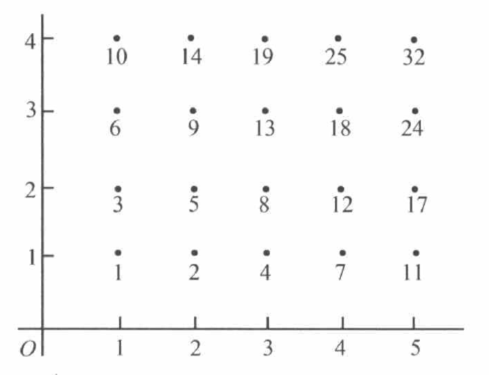
\includegraphics[width=6cm]{attachment/iShot_2023-08-04_15.19.06.png}
	\end{center}
	
	\underline{\textbf{证法二}}~~等价于证明$\mathbb{N}^n$是可数的.构造双射$\sigma : \mathbb{N}^n \to N, ~(\alpha _1,  \cdots , \alpha _n) \mapsto p_1^{\alpha _1} \cdots p_n^{\alpha _n}$.于是$\card \mathbb{N}^n = \card N = \card \mathbb{N}$.
\end{proof}

容易确定: 

\begin{proposition}
	$\card \mathbb{Z} = \card \mathbb{N} = \card \mathbb{Q} = \card \{ x: \exists n \in \mathbb{Z}_+, a_0,  \cdots , a_n \in \mathbb{Z}(a_0+a_1x+\cdots +a_nx^n=0) \}$.
\end{proposition}
\begin{remark}
	最后一个集合意思就是全体代数数构成的集合.
\end{remark}
\begin{proof}
	只证明最后一项.将$n$次整系数多项式的系数提取出来, 做双射于$\Z ^{n+1}$, 可以证明$n$次整系数多项式构成的集合是可数集. 进而所有整系数多项式构成的集合也是可数集. 
	
	利用代数基本定理可以完成后续证明. 
\end{proof}

虽然整数集、有理数集甚至代数数集都是可数的, 我们仍然能找到许多不可数集.

\begin{proposition}{}
	区间$(0, 1)$是不可数的.
\end{proposition}
\begin{proof}
	\underline{\textbf{证法一}}~~(Cantor对角线法) 设$(0, 1)$可数, 记$(0, 1)-\{ x/9: x \in \mathbb{Z},  1 \leq x \leq 8 \}=\{ a_1,  a_2,  \cdots , a_n , \cdots \}$, 并令$a_i$的十进制小数表示为$a_i=0.k_{i1}k_{i2}\cdots$.构作如下无限矩阵: 
	
	$$\begin{pmatrix}
 \color{red} k_{11} & k_{12} & k_{13} & \cdots & k_{1m} & \cdots \\
 k_{21} & \color{red} k_{22} & k_{23} & \cdots & k_{2m} & \cdots \\
 k_{31} & k_{32} & \color{red} k_{33} & \cdots & k_{3m} & \cdots \\
 \vdots & \vdots & \vdots & \color{red} \ddots & \vdots & \cdots \\
 k_{m1} & k_{m2} & k_{m3} & \cdots & \color{red} k_{mm} & \cdots \\
 \vdots & \vdots & \vdots & \vdots & \vdots & \color{red} \ddots
\end{pmatrix}.$$

	选取对角线上的数码$k_{11}, k_{22}, \cdots $.现在任取$k_j \neq k_{jj}$使得$1 \leq k_j \leq 8$.(假设不存在满足不等的$k_j$, 则$a_j$小数点后数码均相同, 必然为$\{ x/9: x \in \mathbb{Z},  1 \leq x \leq 8 \}$中某个元素, 矛盾).
	
	构造$a=0.k_1k_2k_3\cdots$, 由上面的构造可知$a$的十进制小数表示唯一, 又因为存在$m$使得$a=a_m$, 可得$k_m=k_{mm}$, 矛盾.
	
	\underline{\textbf{证法二}}~~之后我们会证明, 可数集一定是零测集(通俗地讲, 就是长度为$0$), 于是$\R$是不可数集. 
\end{proof}



\begin{corollary}{}
	实数集$\R$是不可数的.
\end{corollary}
\begin{remark}
	也可用闭区间套方法证明, 参阅后文. 
\end{remark}
\begin{proof}
	构造函数$f(x)=\tan \ssb{\pi x-\frac{\pi}{2}}$, 易知$f$为$(0, 1)$到$\R$的双射, 故$\card \R = \card (0, 1) > \card \mathbb{N}$.
\end{proof}

现在来看一些常用定理: 

\begin{lemma}{}
	任一无限集均存在可数子集.
\end{lemma}
\begin{proof}
	设无限集$X$, 取其中任意元素$x_0$放入集合$E$.接着在$X-\{ x_0 \}$中取任意元素$x_1$放入$E$.如此重复便得到一可数集$E \subseteq X$.
\end{proof}

\begin{theorem}{}
	无限集与至多可数集的并集与原无限集等势.
\end{theorem}
\begin{proof}
	有限集的情况显然; 考虑无限集$X$与可数集$Y=\{ y_1, y_2, \cdots \}$且$X \cap Y = \varnothing$.由上个引理可知$X$中存在一个可数集$E=\{ x_1, x_2, \cdots \}$.构造映射$f$使得$f(x_j)=x_{2j}, f(y_j)=x_{2j-1},  \forall j \in \mathbb{N}^*$和$f(x)=x, \forall x \in X-E$.容易验证$f$是$X \cup Y \to X$的双射.
\end{proof}

\begin{theorem}{}
	一个集合是无限集等且仅当其包含与自身等势的真子集.(这也被称作Dedekind无限)
\end{theorem}
\begin{proof}
	充分性: 设$X$存在真子集$E$与$X$等势, 假设$X$是有限集, 显然其不可能包含比自己基数大的集合, 矛盾.
	
	必要性: 任取$x \in X$, 可知$E: =X-\{x\}$满足$E \subset X$且$E$与$X$等势.
\end{proof}

从而我们可以证明: 

\begin{proposition}{}
	无理数集与实数集等势. 类似地有超越数(即不是代数数的实数)与实数集等势.
\end{proposition}

\begin{definition}{连续统}
	和实数集$\R$等势的集合称作\textit{连续统}(continuum). 连续统的基数称作\textit{连续基数}, 记作$\aleph _1$.
\end{definition}

一个著名的猜想: 连续统假设. 现在知道, 这个猜想不可能被ZFC公理系统证明或证伪.





